
\subsection{Разработка структуры серверной части конструктора}


В данном разделе описываются разработанные структуры серверной части
конструктора и его основные алгоритмы функционирования.

\subsubsection{Модульная структура серверной части конструктора}

Модуль – набор структур и методов, который обобщает какую-то логику
приложения.

Модульная структура серверной части конструктора представлена на
рисунке~\ref{f:mod-server-struct}.

\begin{figure}[ht]
	\centering
	\vspace{\toppaddingoffigure}
	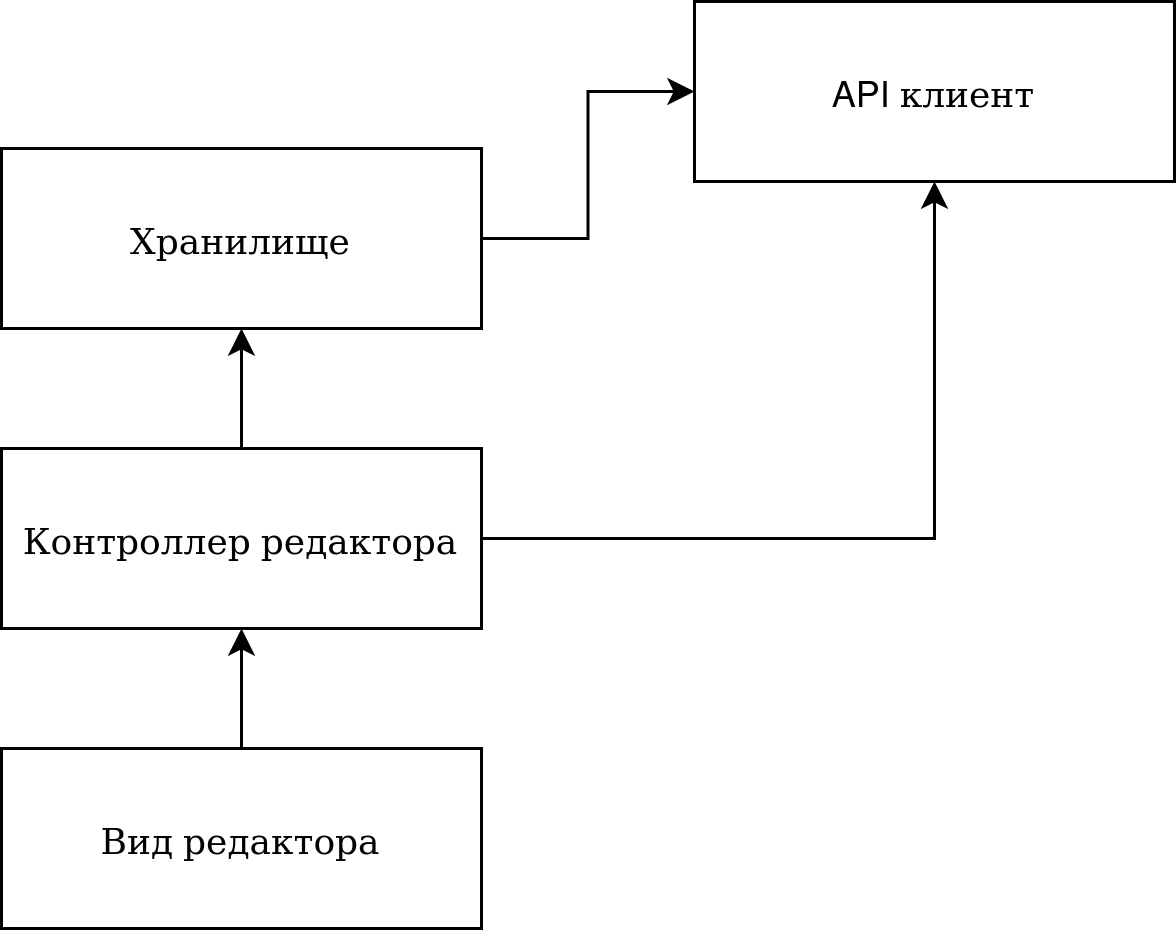
\includegraphics[width=0.8\textwidth]{structures/server/mod}
	\caption{Модульная структура серверной части конструктора}
	\label{f:mod-server-struct}
\end{figure}

Сервис ботов зависит от сервиса пользователей, который предоставляет
первому методы для авторизации пользователя. Также сервис ботов зависит
от модуля компонентов, который описывает структуры компонентов и
реализует их логику выполнения.

Для выполнения логики ботов сервис, обслуживающий ботов, вызывает
методы из модуля компонентов.

\subsubsection{Структура модуля компонентов}

Модуль компонентов состоит из следующих подмодулей:
\begin{itemize}
	\item подмодуль компонентов;
	\item подмодуль контекста;
	\item подмодуль исполнителя;
	\item подмодуль ввода-вывода.
\end{itemize}

Структура модуля компонентов представлена на рисунке~\ref{f:mod-comp-struct}.

\begin{figure}[ht]
	\centering
	\vspace{\toppaddingoffigure}
	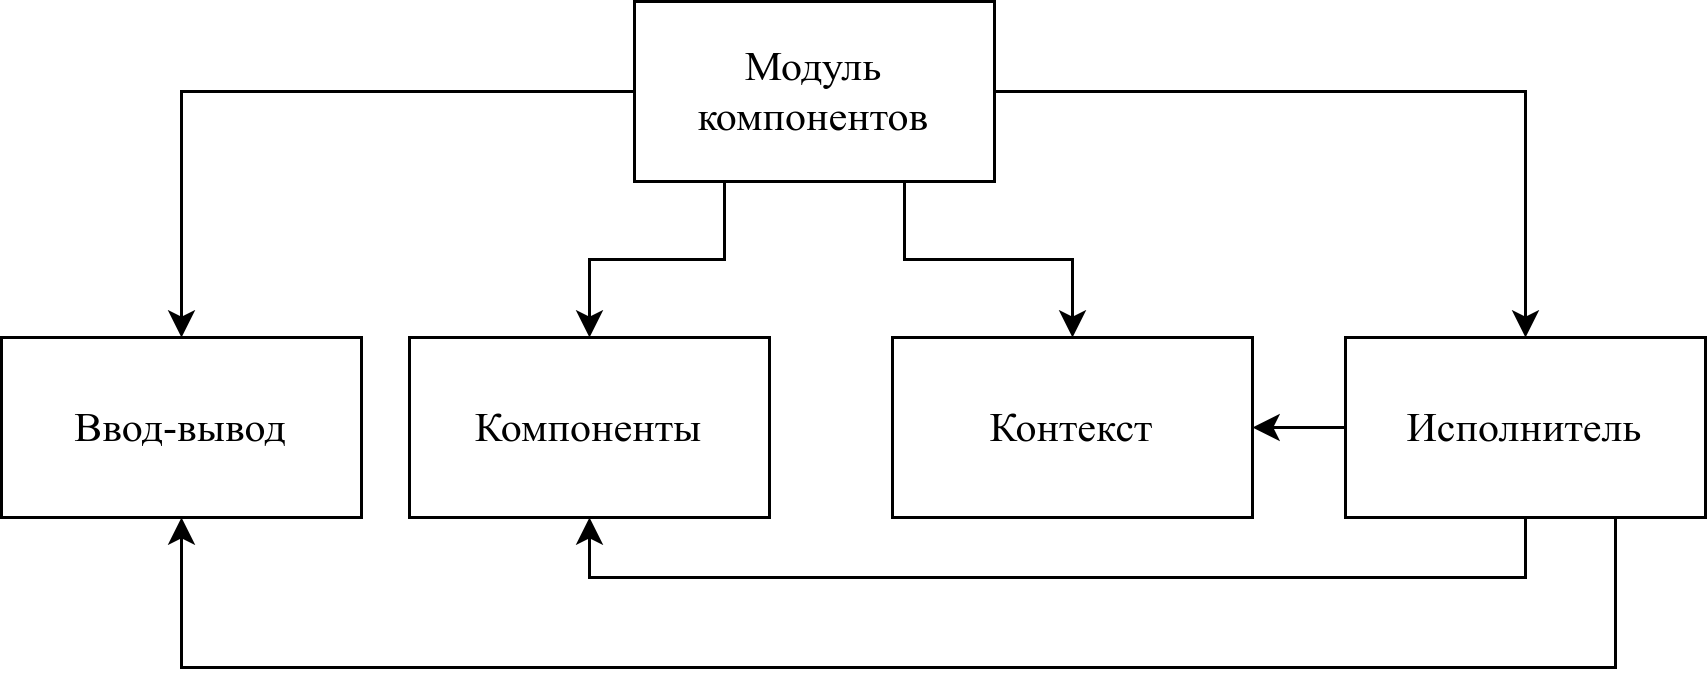
\includegraphics[width=0.8\textwidth]{structures/server/mod-comp}
	\caption{Структура модуля компонентов}
	\label{f:mod-comp-struct}
\end{figure}

Подмодуль компонентов содержит структуру и реализацию логики
компонентов. Каждый компонент реализует общий интерфейс компонента,
который определен в данном подмодуле.

В данном подмодуле определены следующие компоненты:
\begin{itemize}
	\item 	компонент ввода текста;
	\item 	компонент отправки сообщения;
	\item 	компонент вывода кнопок;
	\item 	компонент форматирования;
	\item 	компонент точки входа;
	\item 	компонент условия.
\end{itemize}

Подмодуль ввода-вывода предоставляет интерфейс, через который
окружение обменивается данными с рядом компонентов.

Подмодуль контекста содержит методы для работы с контекстом.
Контекст в рамках бота – память, с которой работают компоненты:
компоненты получают из контекста данные для выполнения и записывают в
него результат.

Исполнитель представляет собой объект, который содержит в себе
контекст и интерфейс ввода-вывода. Через него происходит выполнение
компонентов.


\subsubsection{Алгоритмы функционирования серверной части конструктора}

Пользователь конструктора взаимодействует с сервисом ботом, который
контролирует изменение данных и состояние ботов.
Схема алгоритма обработки запросов от пользователей сервиса ботов
представлен на рисунке~\ref{f:bot-service-alg}.

\begin{figure}[hp]
	\centering
	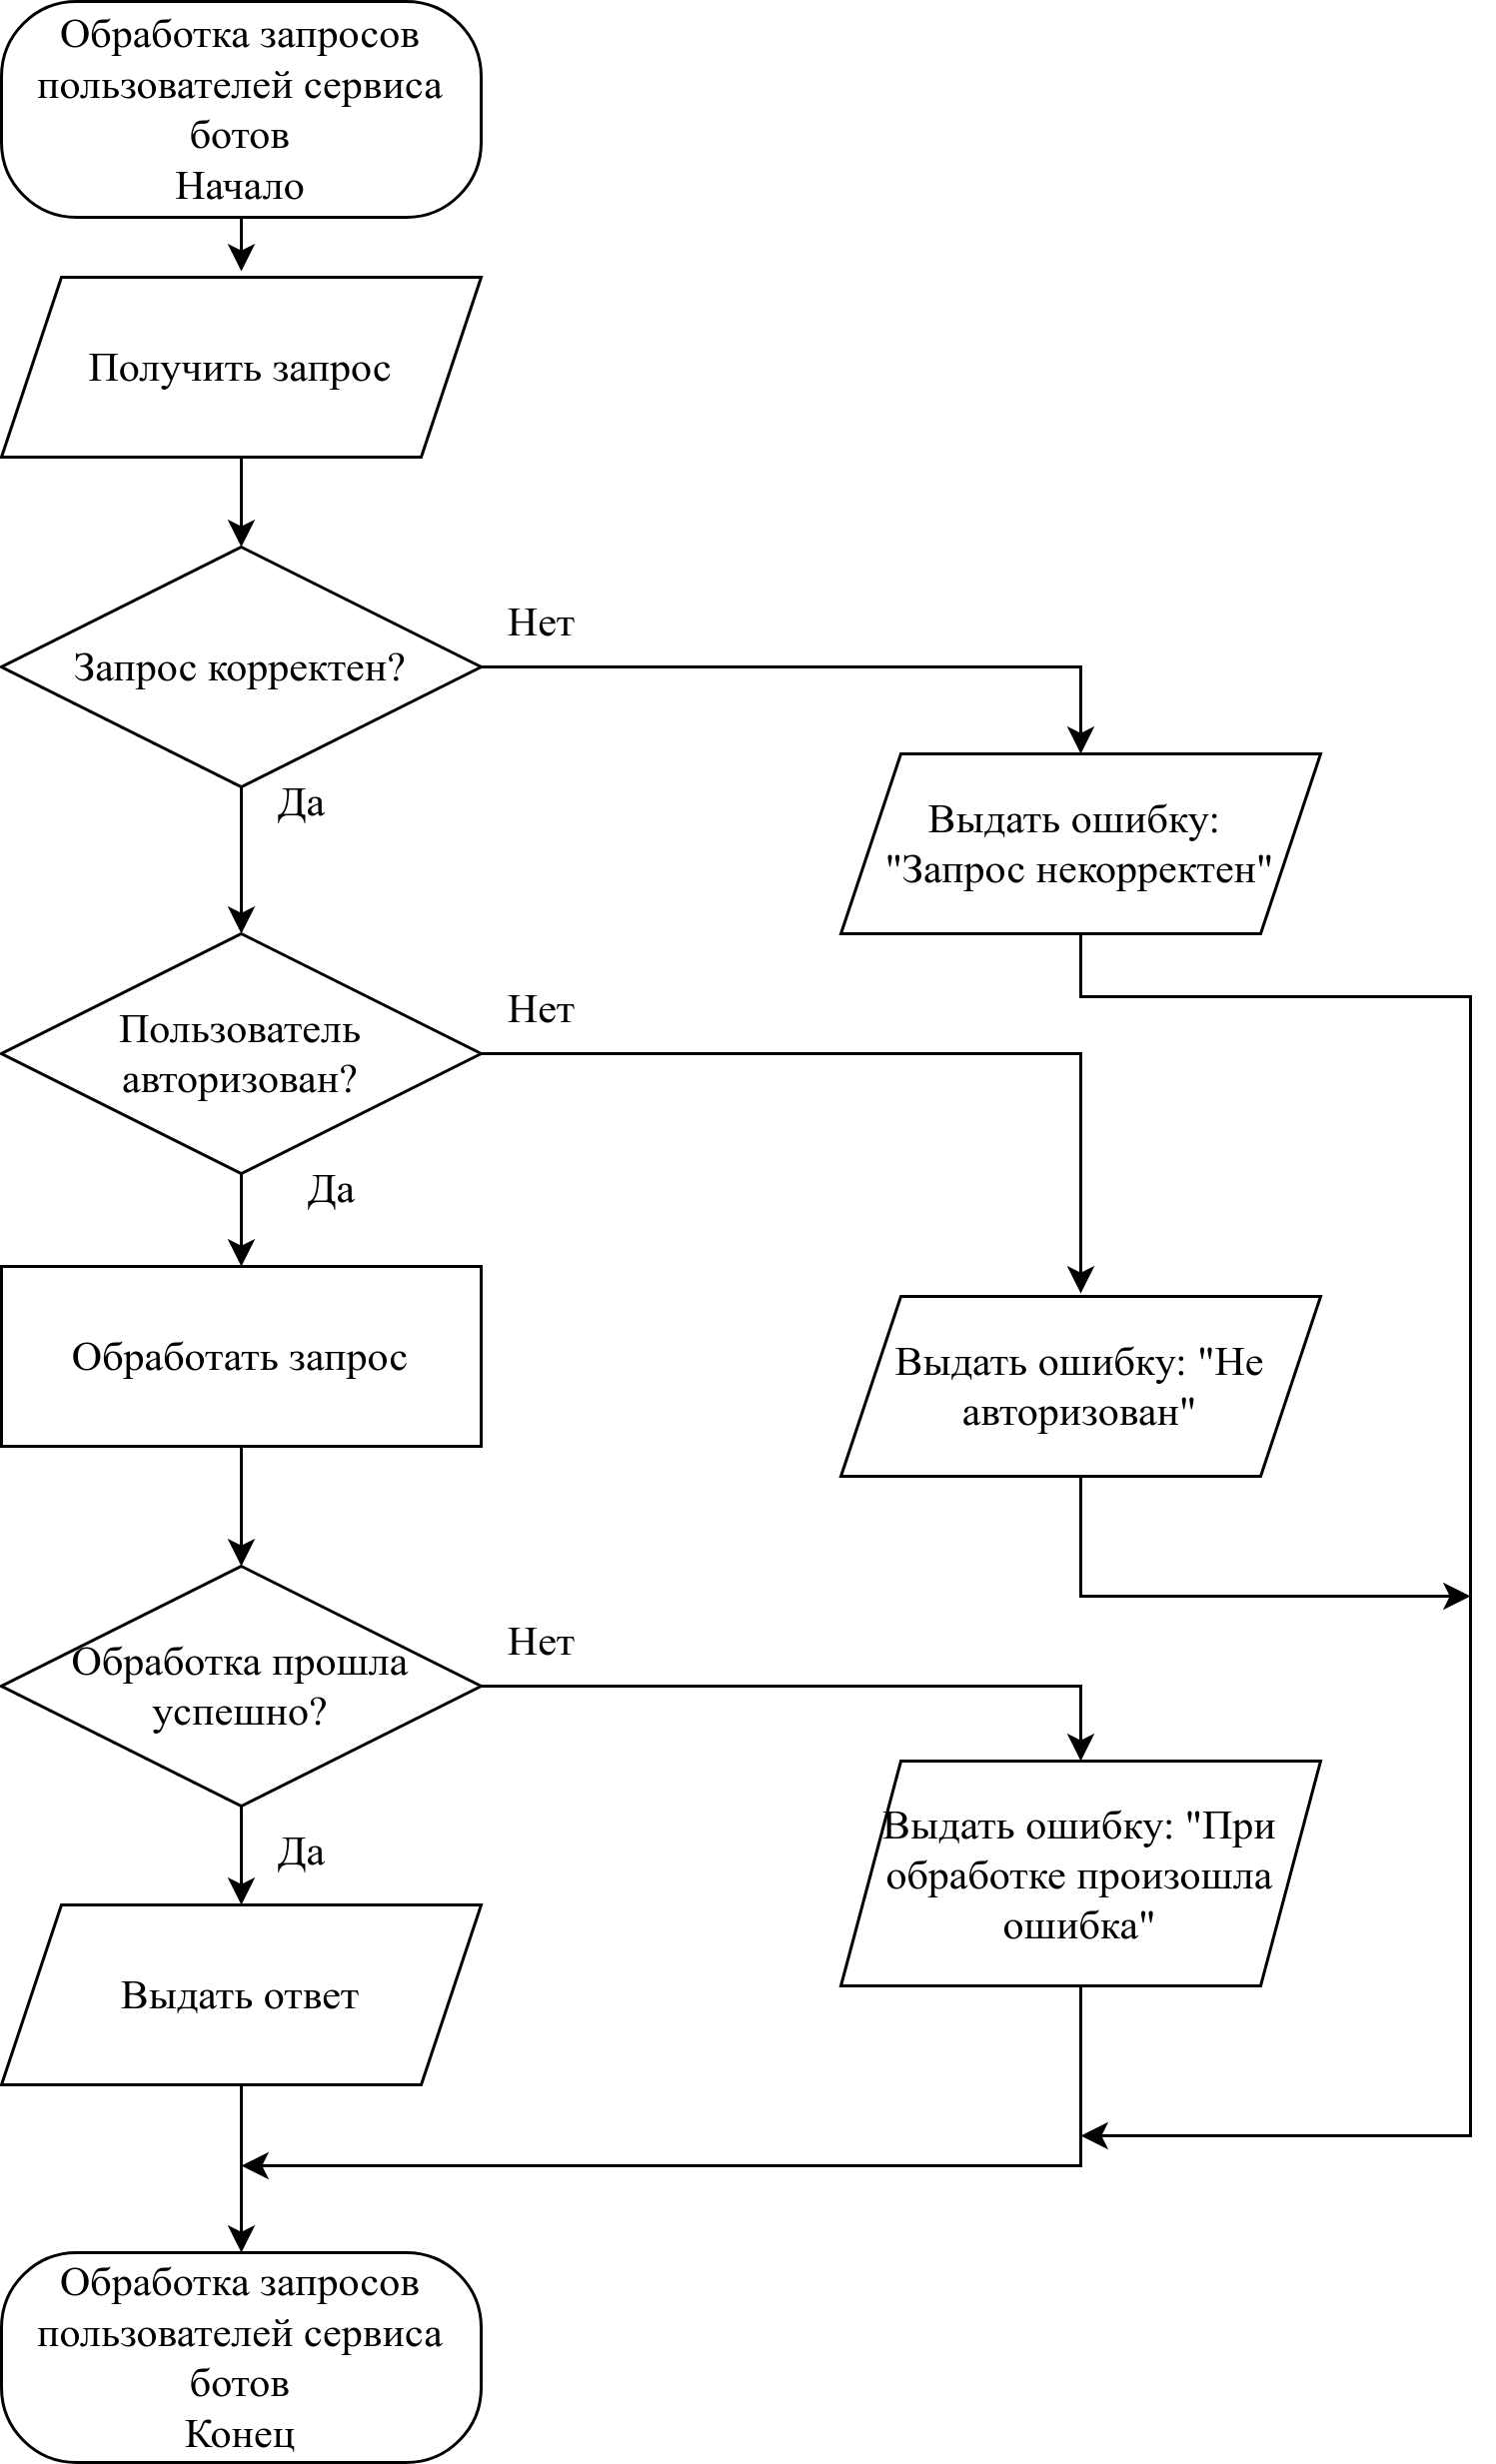
\includegraphics[height=0.9\textheight]{bot-service-alg}
	\caption{Схема алгоритма обработки запросов от пользователей сервиса ботов}
	\label{f:bot-service-alg}
\end{figure}

При получении запроса проверяется его корректность.
Если запрос не корректен, например, такое обращение не доступно, то
выводится соответствующая ошибка. Чтобы обработка прошла успешно, пользователь
должен быть авторизован в системе. В случае успешной обработки запроса выдается
ответ, иначе - ошибка.


При взаимодействии Telegram пользователя с ботом происходит
отправка запросов сервису, обслуживающему ботов, который в дальнейшем
обрабатывает данное событие. Схема алгоритма обработки запросов от
пользователя бота представлен на рисунке~\ref{f:bot-worker-alg}.


\begin{figure}[hp]
	\centering
	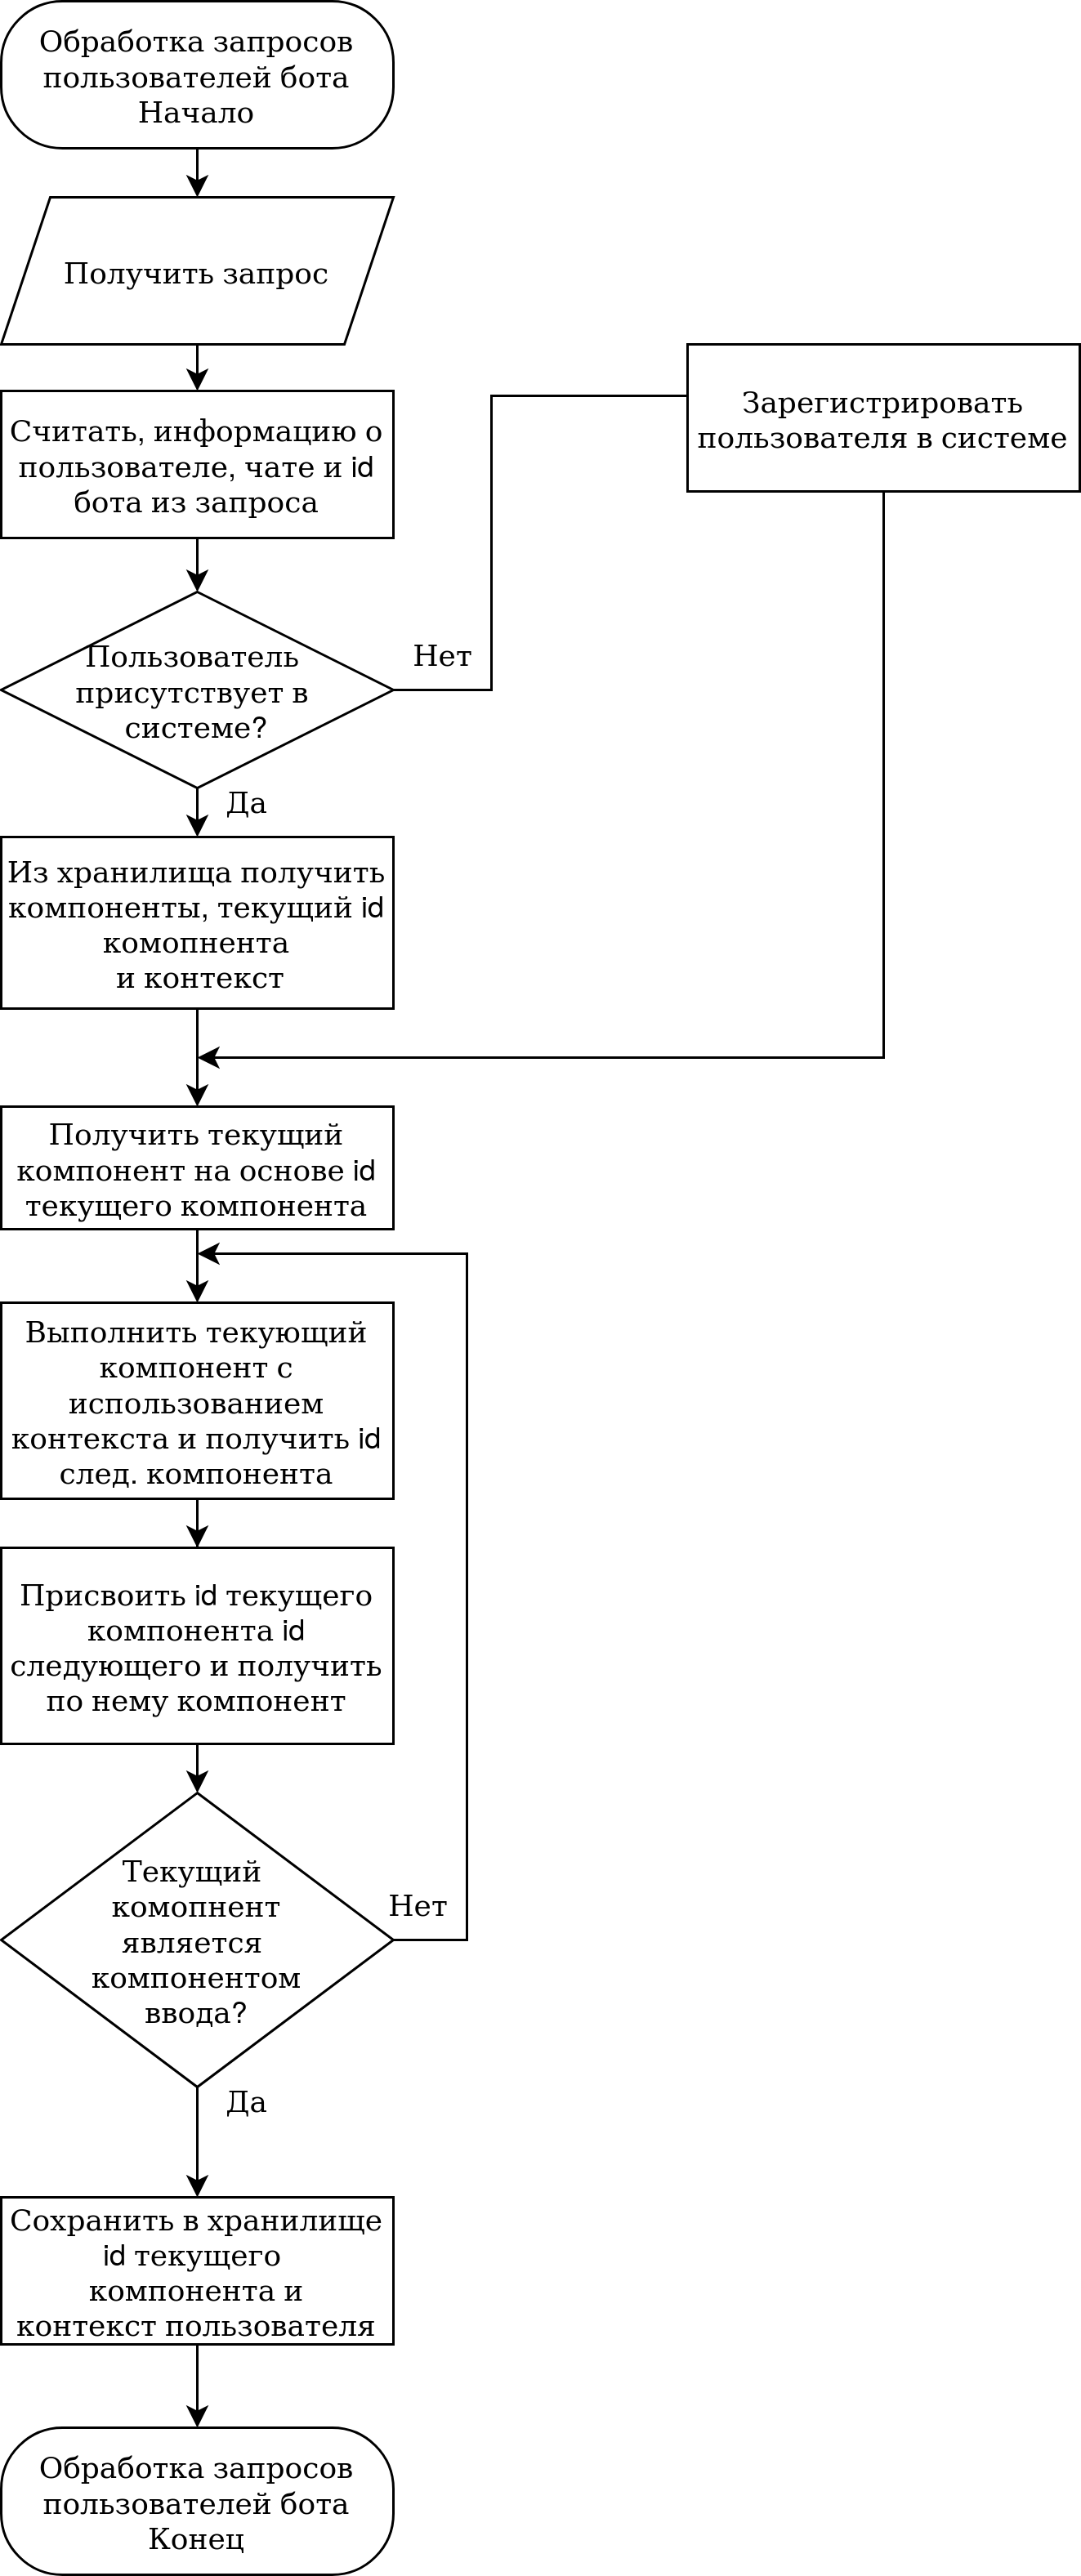
\includegraphics[height=0.9\textheight]{bot-worker-alg}
	\caption{Схема алгоритма обработки запросов от пользователей ботов}
	\label{f:bot-worker-alg}
\end{figure}

При принятии события сервисом происходит считывание следующих
данных:
\begin{itemize}
	\item информация о пользователе;
	\item информация о чате;
	\item id бота, от которого пришло сообщение.
\end{itemize}

На основе этих данных из хранилища идёт получение следующих
данных:
\begin{itemize}
	\item контекст пользователя;
	\item id текущего компонента пользователя;
	\item компонентов бота.
\end{itemize}

На основании id текущего компонента происходит получение текущего
компонента, который затем выполняется. Результат выполнения представляет
собой id следующего компонента, который присваивается текущему.

На основании следующего компонента принимается решение: если
компонент ожидает ввода каких-либо данных, то алгоритм заканчивается с
сохранением контекста и id текущего компонента, иначе идет выполнение
следующего компонента.

\newpage


\subsubsection{Обеспечение защиты информации клиентов конструктора}

Для обеспечения защищенного хранения паролей в базе данных используется
адаптивная криптографическая хеш-функция bcrypt \refref{ref:bcrypt}.

Функция основана на шифре Blowfish.
Для защиты от атак с помощью радужных таблиц bcrypt использует соль (salt);
кроме того, функция является адаптивной,
время её работы легко настраивается и её можно замедлить,
чтобы усложнить атаку перебором \refref{ref:bcrypt}.

Функция принимает три параметра: стоимость(cost), соль и пароль.
Алгоритм хеширования состоит из следующих шагов \refref{ref:bcrypt}:
\begin{enumerate}
	\item
	      инициализация состояния Blowfish с помощью дорогостоящего алгоритма настройки ключей;
	      результат состоит из массива P, состоящего из 18 подключей, и четырех S-боксов;
	\item шифрование текста «OrpheanBeholderScryDoubt» 64 раза с помощью стандартного
	      Blowfish в режиме простой замены;
	\item результат состоит из конкатенации стоимости, соли и зашифрованного текста
	      «OrpheanBeholderScryDoubt».

\end{enumerate}

Дорогостоящий алгоритм настройки ключей включает в себя следующие шаги
\refref{ref:bcrypt}:
\begin{enumerate}
	\item инициализация подключей P и S-боксов шестнадцатеричными цифрами числа $\pi$;
	\item перестановка P и S на основе пароля и соли: ExpandKey(P, S, password, salt);
	\item повторение $2^{cost}$ раз следующих шагов:
	      \begin{enumerate}
		      \item перестановка P и S на основе пароля: ExpandKey(P, S, password, 0);
		      \item перестановка P и S на основе соли: ExpandKey(P, S, salt, 0).
	      \end{enumerate}
\end{enumerate}

Алгоритм ExpendKey
\refref{ref:bcrypt}:
\begin{enumerate}
	\item смешивание пароля с массивом подключей P;
	\item
	      разбиение соли на две равные части;
	\item инициализация буфера для хранения блоков;
	\item циклическое смешивание внутреннего состояния с P, используя половины соли;
	\item циклическое смешивание зашифрованного состояния с внутренними S-блоками состояния,
	      используя половины соли.
\end{enumerate}

Аутентификация пользователя происходит по паролю и логину.
Отправленный пароль после хеширования
сравнивается с хешем из базы данных, и в случае успеха генерируется токен доступа.
Этот токен временно сохраняется в базе данных, а его копия выдается пользователю.
Используя токен, пользователь может получать доступ к функциям сервиса ботов.


